\documentclass[dvipdfmx,11pt,notheorems]{beamer}
%%%% 和文用 %%%%%
\usepackage{bxdpx-beamer}
\usepackage{pxjahyper}
\usepackage{minijs}%和文用
\usepackage{listings,jlisting} % プログラムの表示用
\usepackage{type1cm}
\renewcommand{\kanjifamilydefault}{\gtdefault}%和文用

%%%% tikz 用 %%%%%
\usepackage[latin1]{inputenc}
\usepackage{tikz}
\usetikzlibrary{intersections}
\usetikzlibrary{shapes,arrows}

%%%% スライドの見た目 %%%%%
\usetheme{Boadilla}
\usecolortheme{seahorse}
\usefonttheme{professionalfonts}
\setbeamertemplate{frametitle}[default][center]
\setbeamertemplate{navigation symbols}{}
\setbeamercovered{transparent}%好みに応じてどうぞ)
\setbeamertemplate{footline}[page number]
\setbeamerfont{footline}{size=\normalsize,series=\bfseries}
\setbeamercolor{footline}{fg=black,bg=black}

\setbeamercolor{white-cyan1}
{fg=white,bg=cyan!80!black}
\setbeamercolor{white-cyan2}
{fg=white,bg=cyan!60!black}

%フラットデザイン化
\setbeamertemplate{blocks}[rounded] % Blockの影を消す
%Beamer色設定
\definecolor{UniBlue}{RGB}{0,150,200}
\definecolor{AlertOrange}{RGB}{255,76,0}
\definecolor{AlmostBlack}{RGB}{38,38,38}
\setbeamercolor{structure}{fg=UniBlue} % 見出しカラー
\setbeamercolor{block title}{fg=UniBlue!50!black} % ブロック部分タイトルカラー
%%%%

%%%% 定義環境 %%%%%
\usepackage{amsmath,amssymb}
\usepackage{amsthm}
\usepackage{bm}
\theoremstyle{definition}
\newtheorem{theorem}{定理}
\newtheorem{definition}{定義}
\newtheorem{proposition}{命題}
\newtheorem{lemma}{補題}
\newtheorem{corollary}{系}
\newtheorem{conjecture}{予想}
\newtheorem*{remark}{Remark}
\renewcommand{\proofname}{}
%%%%%%%%%

%%%%% フォント基本設定 %%%%%
% \usepackage[T1]{fontenc}%8bit フォント
% \usepackage{textcomp}%欧文フォントの追加
% \usepackage[utf8]{inputenc}%文字コードをUTF-8
% \usepackage{otf}%otfパッケージ
% \usepackage{lxfonts}%数式・英文ローマン体を Lxfont にする
% \usepackage{bm}%数式太字
%%%%%%%%%%

%%%%% 複数人の著者を揃える %%%%%
%% http://tex.stackexchange.com/questions/
%%   166531/how-to-change-author-alignment-in-beamer
\makeatletter
\long\def\beamer@author[#1]#2{%
  \def\insertauthor{\def\inst{\beamer@insttitle}\def\and{\beamer@andtitle}%
  \begin{tabular}{rl}#2\end{tabular}}%
  \def\beamer@shortauthor{#1}%
  \ifbeamer@autopdfinfo%
    \def\beamer@andstripped{}%
    \beamer@stripands#1 \and\relax
    {\let\inst=\@gobble\let\thanks=\@gobble\def\and{, }\hypersetup{pdfauthor={\beamer@andstripped}}}
  \fi%
}
\makeatother
%%%%%%%%%%

%%%%% プログラムに色をつける
\usepackage{color}

\definecolor{codegreen}{rgb}{0,0.6,0}
\definecolor{codegray}{rgb}{0.5,0.5,0.5}
\definecolor{codepurple}{rgb}{0.58,0,0.82}
\definecolor{backcolour}{rgb}{0.95,0.95,0.92}

\lstdefinestyle{mystyle}{
    backgroundcolor=\color{backcolour},
    commentstyle=\color{codegreen},
    keywordstyle=\color{magenta},
    numberstyle=\tiny\color{codegray},
    stringstyle=\color{codepurple},
    basicstyle=\footnotesize,
    breakatwhitespace=false,
    breaklines=true,
    captionpos=b,
    keepspaces=true,
    numbers=left,
    numbersep=5pt,
    showspaces=false,
    showstringspaces=false,
    showtabs=false,
    tabsize=2
}

\lstset{style=mystyle}

%%%%
\title[略タイトル]{第4回 知能システム学特論レポート}%[略タイトル]{タイトル}
\author[NishidaLab]{
15344203 & 有田 裕太 \\
15344206 & 緒形 裕太 \\
15344209 & 株丹 亮 \\
12104125 & 宮本 和 }%[略名前]{名前}
\institute[NishidaLab]{西田研究室,計算力学研究室}%[略所属]{所属}
\date{2015年\ 7月\ 2日}%日付

\begin{document}

%%%% 1 %%%%
\begin{frame}[plain]\frametitle{}
\titlepage %表紙
\end{frame}

% \begin{frame}\frametitle{Contents}
% \tableofcontents %目次
% \end{frame}

%%%% 進捗状況 %%%%
\begin{frame}\frametitle{進捗状況}

\begin{block}{理論研究の進捗}
畳込みニューラルネットワークの理論について
\end{block}

\vspace{1cm}
\begin{exampleblock}{プログラミングの進捗}
中間層の出力,可視化
\end{exampleblock}
\end{frame}


%%%% 畳込みニューラルネットワーク %%%%
\begin{frame}[fragile]\frametitle{畳込みニューラルネットワーク}
\begin{itemize}
\item 畳込みニューラルネットワークは主に画像認識に応用される順伝播型ニューラルネットワークである.
\item 順伝播型ネットワークは隣接層間のユニットの全てが結合されているのに対し,畳込みニューラルネットワークでは特定のユニットのみが結合を持つ特別な構造を持つ.
\item 神経細胞はその受容野に刺激が入った場合にのみ反応し、受容野の外側にいくら刺激を与えても、細胞を発火しないという特徴を持つ.
\end{itemize}

\begin{figure}[htbp]
  \begin{center}
   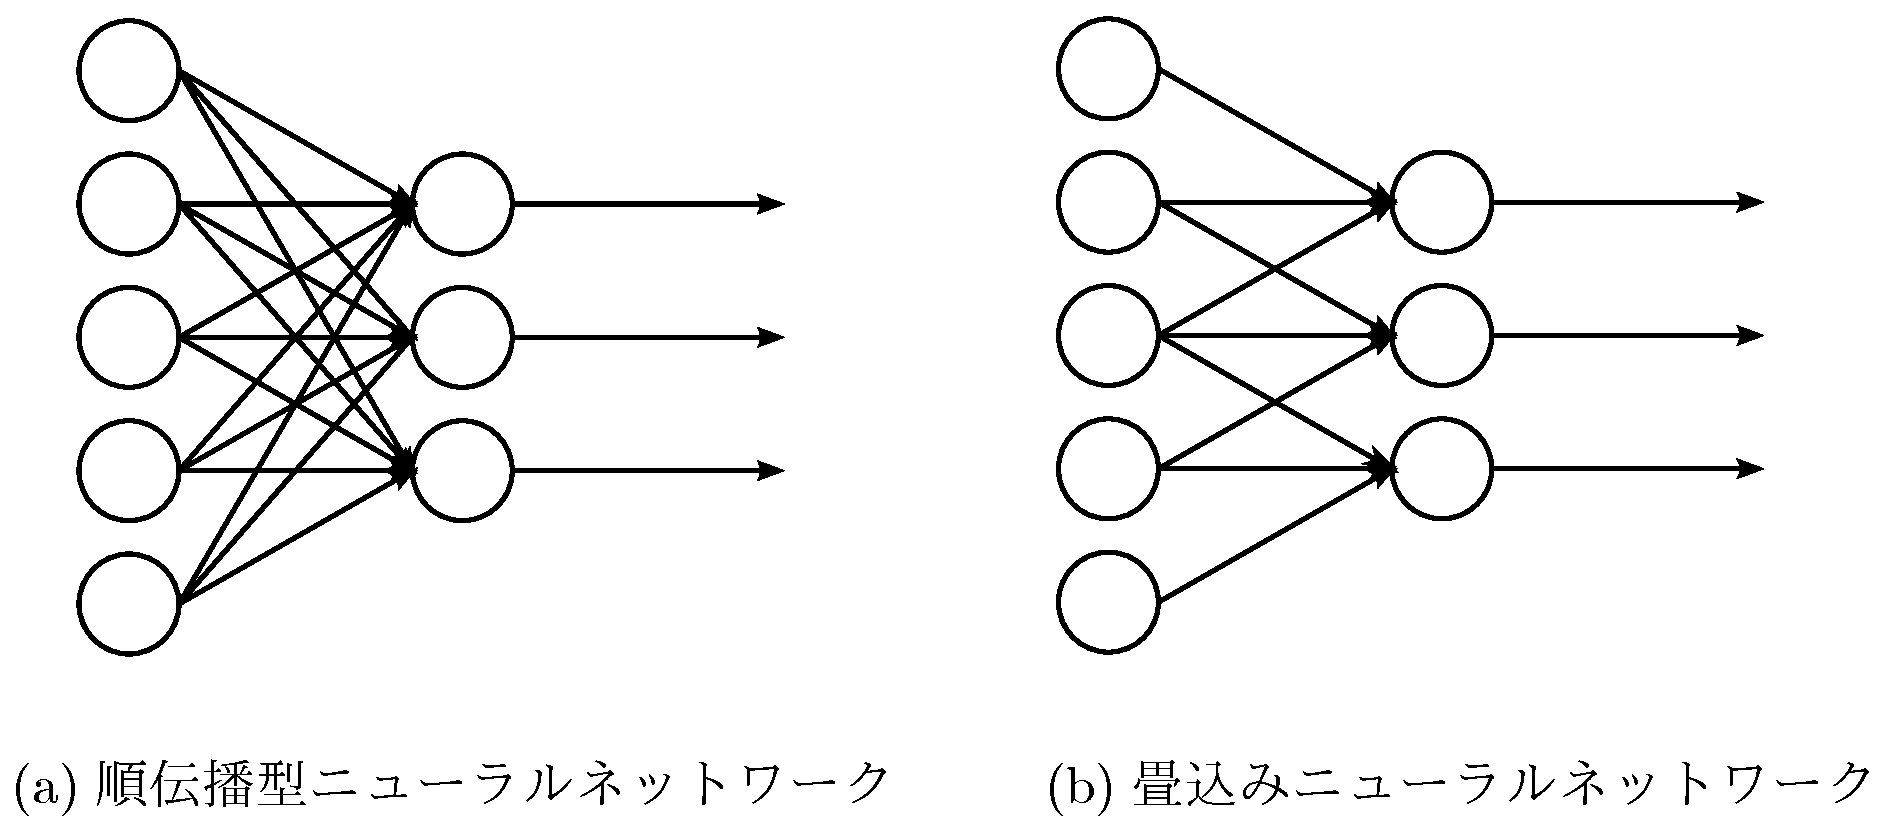
\includegraphics[width=70mm]{fig/eps/network.eps}
  \end{center}
  \caption{畳込みニューラルネットワーク}
  \label{fig:FNN}
\end{figure}
\end{frame}


%%%% 単純型細胞と複雑型細胞 1 %%%%
\begin{frame}[fragile]\frametitle{単純型細胞と複雑型細胞}
\begin{figure}[t]
 \centering
 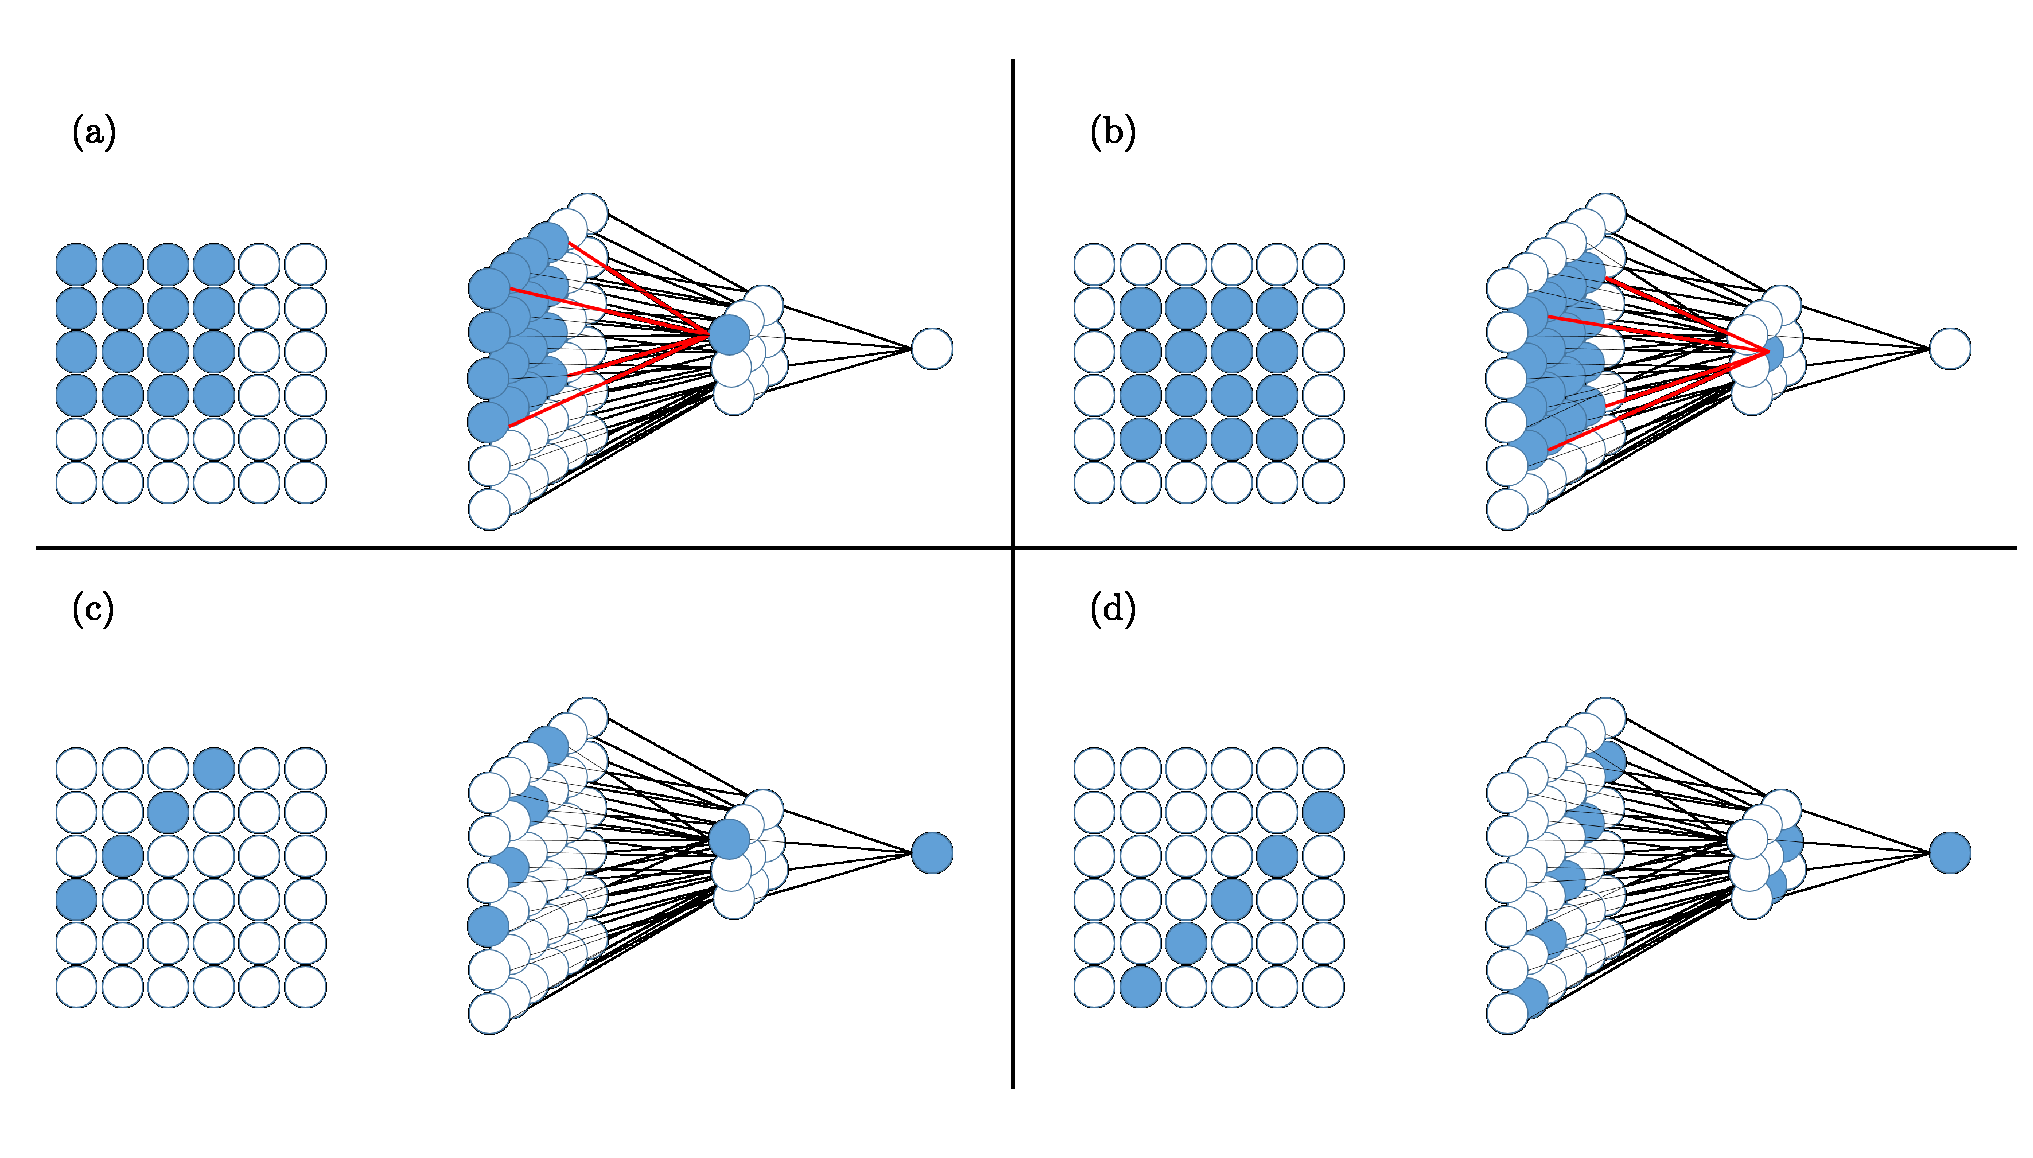
\includegraphics[scale=0.3]{fig/eps/cnn62.eps}
    \caption{単純型細胞と複雑型細胞のモデル}
    \label{fig:単純型細胞と複雑型細胞のモデル}
\end{figure}

\begin{itemize}
\item (a),(b) 入力層と中間層の結合
\item (c),(d) 中間層の変化と出力層の変化
\end{itemize}

\end{frame}

%%%% 単純型細胞と複雑型細胞 2 %%%%
\begin{frame}[fragile]\frametitle{単純型細胞と複雑型細胞}
\begin{itemize}
\item 2つの細胞をモデル化した二層構造を繰り返す構造がCNNに用いられている
\item 神経科学の分野において,多層のCNNが霊長類の脳の高次視覚野と似た振る舞いを示す
\item コンピュータによる物体カテゴリ認識ができるようになってきている
\end{itemize}
\end{frame}


%%%% 畳込みニューラルネットワークの構造 1 %%%%
\begin{frame}[fragile]\frametitle{畳込みニューラルネットワークの構造}

\begin{figure}[tb]
  \begin{center}
    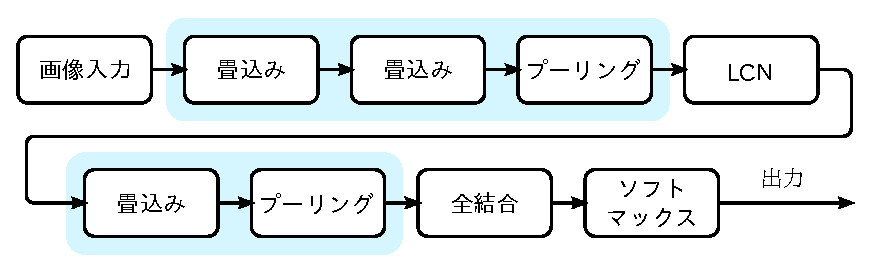
\includegraphics[clip,width=9cm]{fig/eps/structure.eps}
  \end{center}
  \caption{畳込みニューラルネットワークの構造}
\end{figure}

\begin{itemize}
\item 畳込み層(convolution layer)とプーリング層(pooling layer)が\\ペアでこの順に並び,このペアが複数回繰り返される
\item 畳込み層とプーリング層の後に,局所コントラスト正規化\\(local contrast normalization, LCN)層を挿入する場合がある
\item 畳込み層とプーリング層の繰り返しの後には,隣接層間ユニットが\\全結合した層が配置される
\item 目的がクラス分類であれば最終的な出力はソフトマックスを適用する
\end{itemize}
\end{frame}

%%%% 畳込みニューラルネットワークの構造 2 %%%%
\begin{frame}[fragile]\frametitle{畳込みニューラルネットワークの構造}

\begin{figure}[tb]
  \begin{center}
    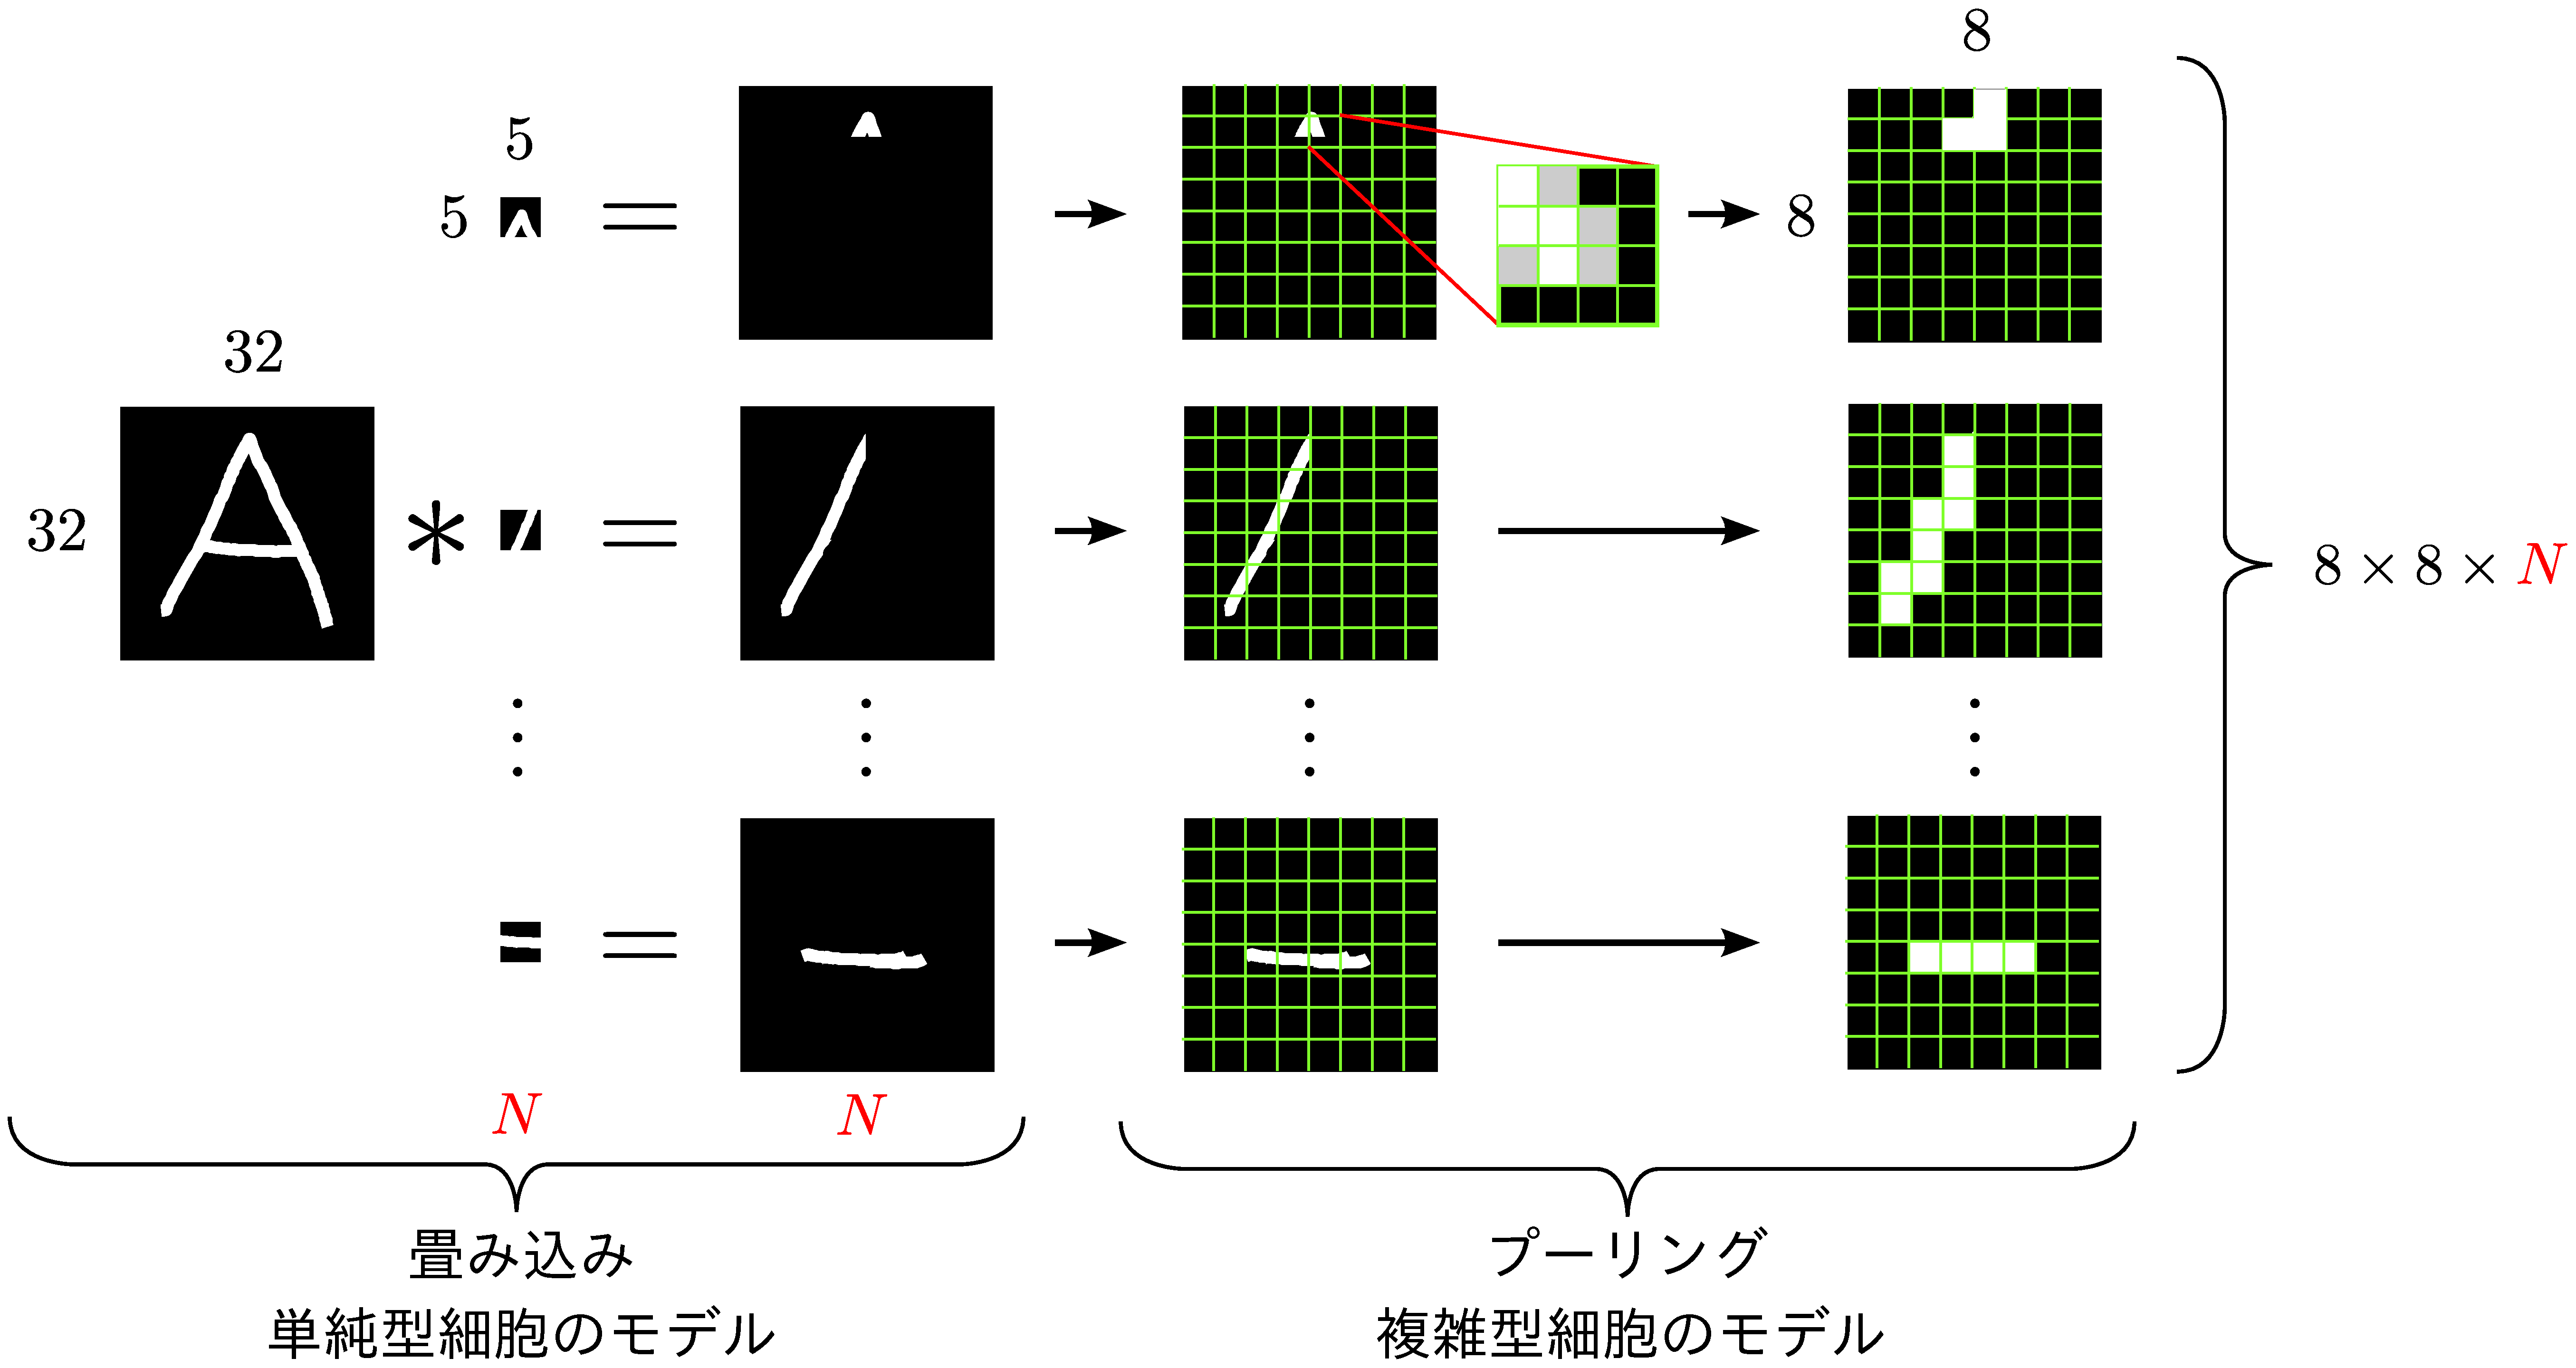
\includegraphics[clip,width=12cm]{fig/eps/conv_pool.eps}
  \end{center}
  % \caption{畳込みニューラルネットワークの構造}
\end{figure}
\end{frame}

%%%% 畳込みニューラルネットワークの構造 2 %%%%
\begin{frame}[fragile]\frametitle{畳込みニューラルネットワークの構造}

\begin{figure}[tb]
  \begin{center}
    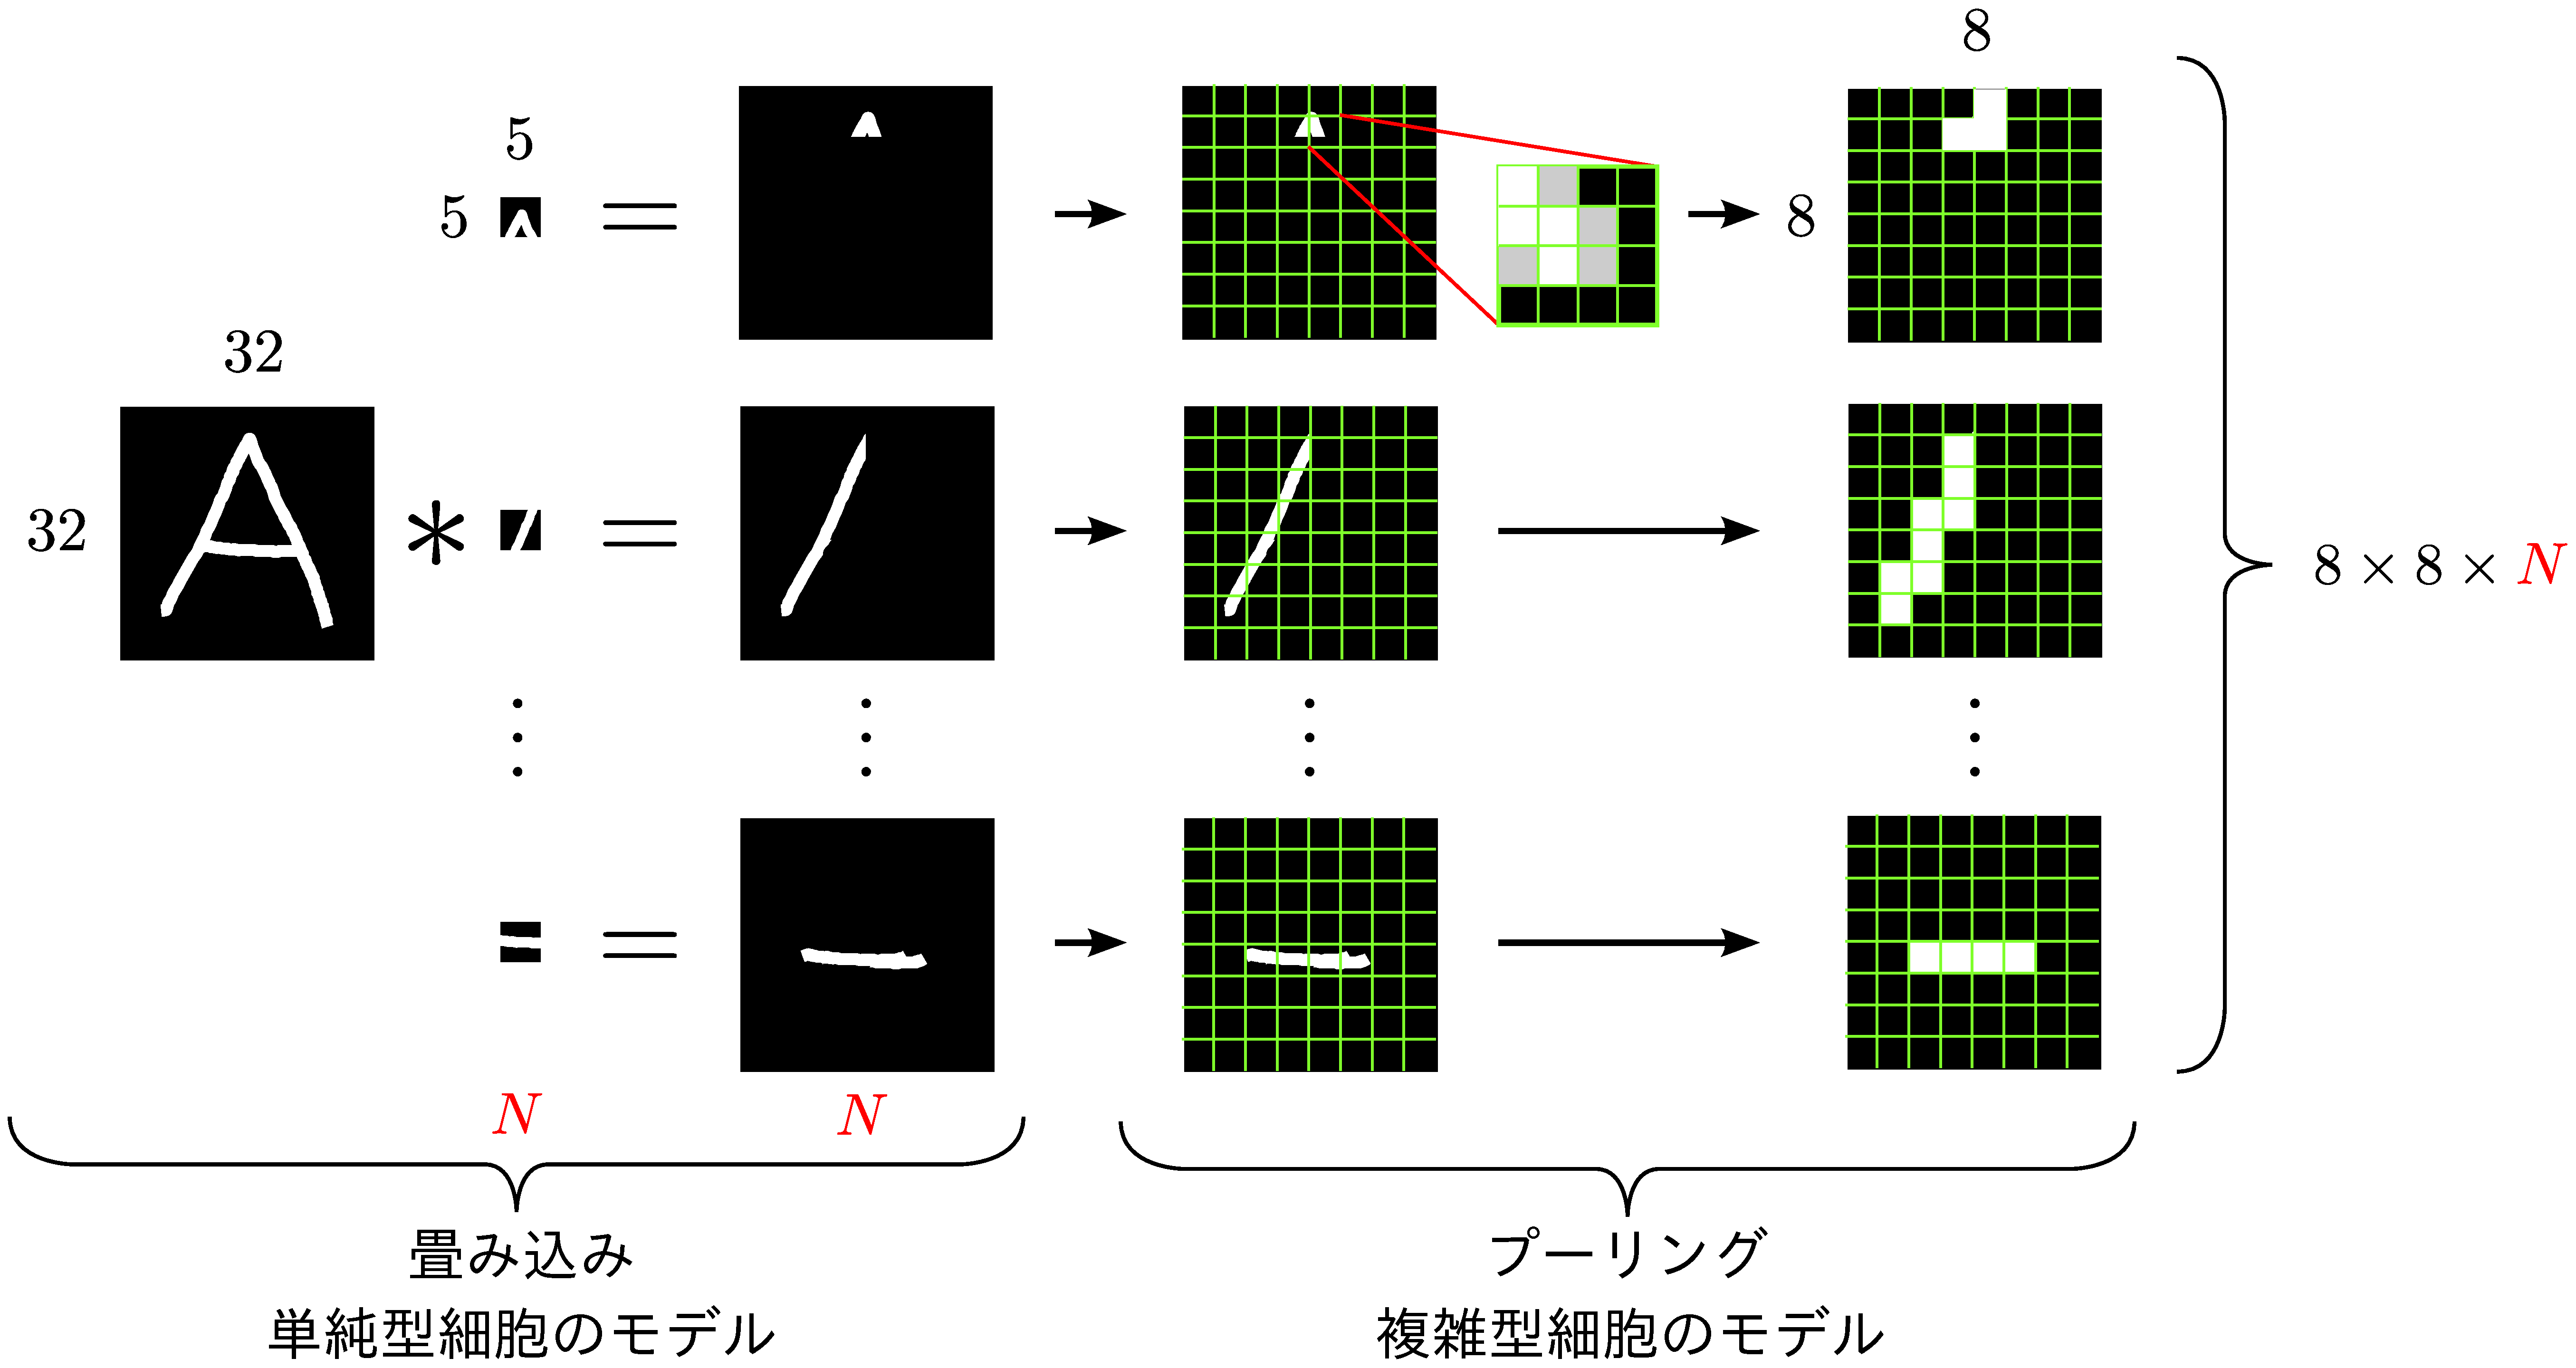
\includegraphics[clip,width=10cm]{fig/eps/conv_pool.eps}
  \end{center}
  % \caption{畳込みニューラルネットワークの構造}
\end{figure}

\begin{block}{二層の働き}
\begin{itemize}
\item 畳込み層はフィルタが表す特徴を入力から抽出する
\item プーリング層は抽出された特徴の位置感度を低下させる
\end{itemize}
\end{block}

\end{frame}


%%%% プログラム 1 %%%%
\begin{frame}\frametitle{プログラム}
\begin{block}{caffeNetの構造}
caffeNetは5つの畳込み層,3つのプーリング層,2つの正規化層,そして3つの全結合層からできている.また活性化関数にはソフトマックス関数を用いている.
\end{block}
\vspace{0.2cm}
\begin{figure}[tb]
  \begin{center}
    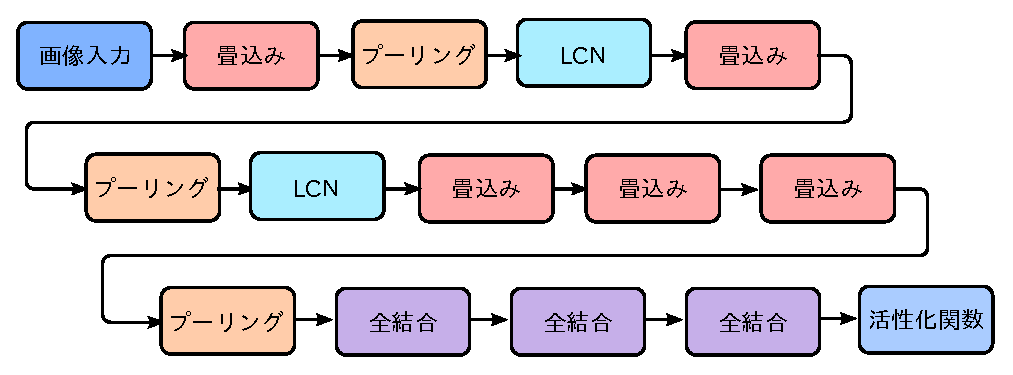
\includegraphics[clip,width=12cm]{fig/eps/caffeNet_structure.eps}
  \end{center}
   \caption{caffeNetの構造}
\end{figure}
\vspace{0.2cm}
\end{frame}

%%%% プログラム 2 %%%%
\begin{frame}\frametitle{プログラム}
\begin{block}{中間層の出力}
畳込み1層目のフィルタと図に示す入力画像を入力したときの出力を得ることができた.畳込み1層目は全部で96個の$11\times11$のフィルタから構成されており,ストライドが4である.従って,出力される画像のサイズは$55\times55$であり,96個の画像が出力される.
\end{block}
\begin{figure}[tb]
  \begin{center}
    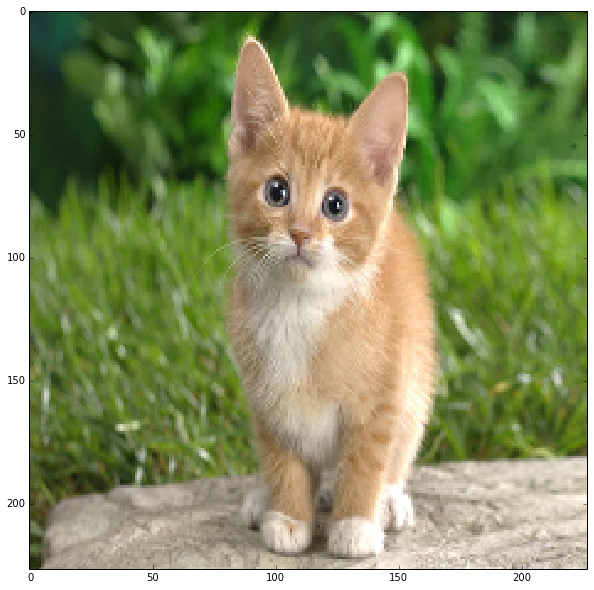
\includegraphics[clip,width=4.5cm,bb=0 0 594 590]{./fig/png/input.png}
  \end{center}
   \caption{入力画像}
\end{figure}
\end{frame}

%%%% プログラム 3 %%%%
\begin{frame}\frametitle{プログラム}

\begin{figure}[t]
 \begin{minipage}{0.4\hsize}
  \centering
  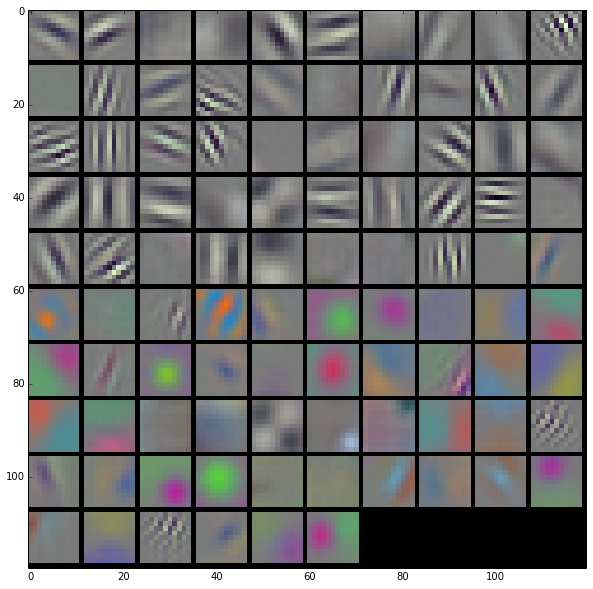
\includegraphics[width=50mm,bb=0 0 594 590]{./fig/png/conv1_params.png}
  \caption{フィルタ}
 \end{minipage}
 \begin{minipage}{0.4\hsize}
  \centering
  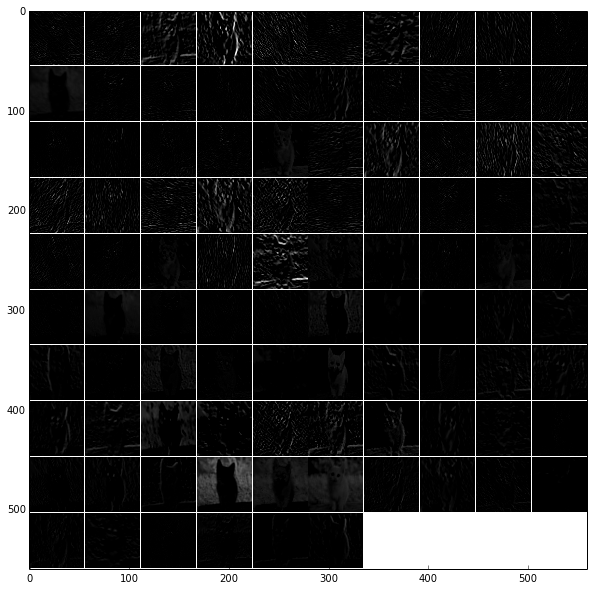
\includegraphics[width=50mm,bb=0 0 594 590]{./fig/png/conv1_blobs.png}
  \caption{フィルタの出力}
 \end{minipage}
\end{figure}
\end{frame}

%%%% 今後の課題 %%%%
\begin{frame}\frametitle{今後の課題}

\begin{block}{理論研究}
CNNの詳細な調査\\
畳み込み,プーリングの理論
\end{block}

\vspace{1cm}
\begin{exampleblock}{プログラミング}
データセットの作成
\end{exampleblock}
\end{frame}

% \begin{figure}[t]
%  \begin{minipage}{0.3\hsize}
%   \centering
%   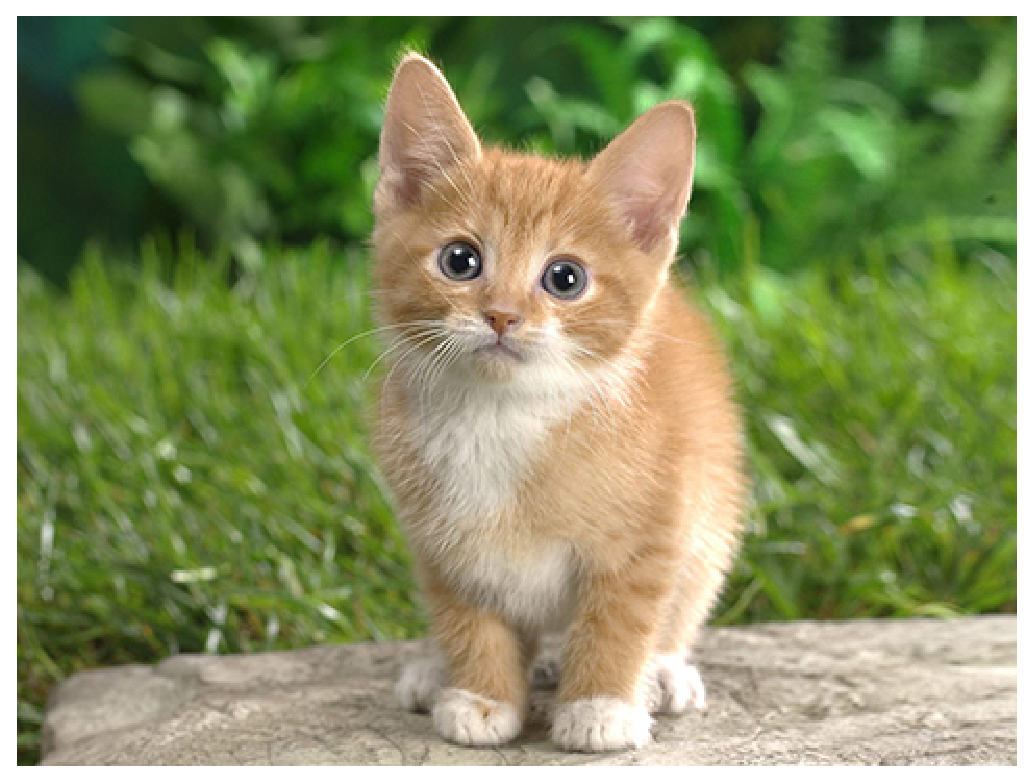
\includegraphics[width=30mm]{./figure/cat.eps}
%   \caption{cat.jpg}
%   \label{sample1}
%  \end{minipage}
%  \begin{minipage}{0.3\hsize}
%   \centering
%   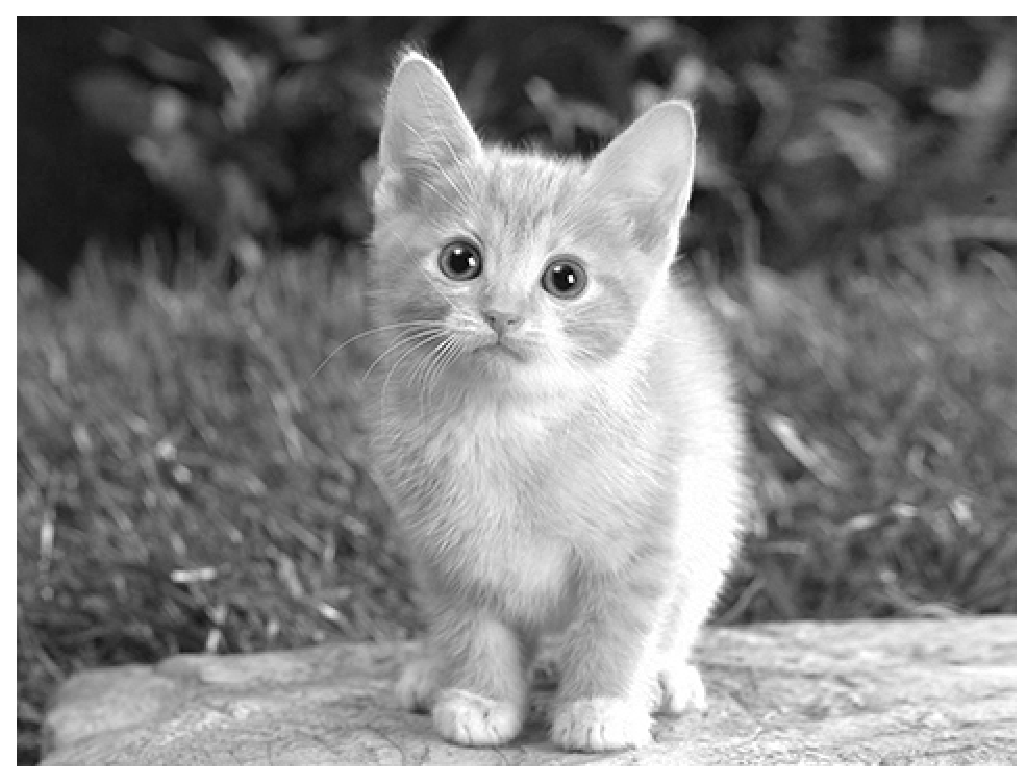
\includegraphics[width=30mm]{./figure/cat_gray.eps}
%   \caption{cat\_gray.jpg}
%   \label{sample2}
%  \end{minipage}
%  \begin{minipage}{0.3\hsize}
%   \centering
%   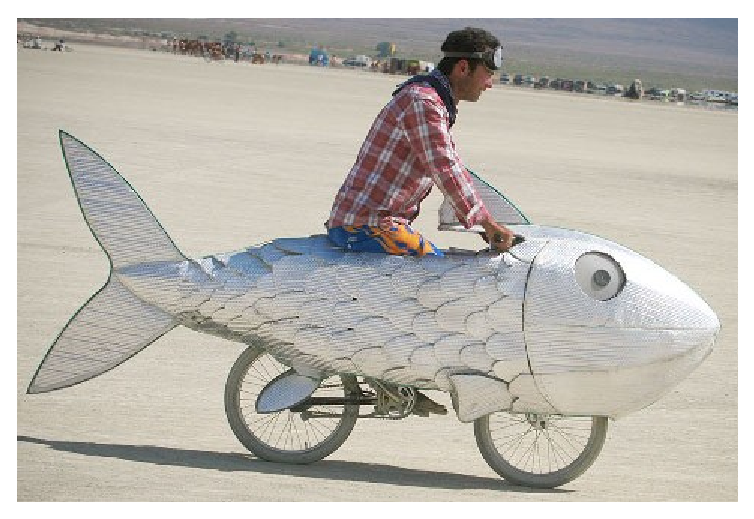
\includegraphics[width=30mm]{./figure/fish-bike.eps}
%   \caption{fish-bike.jpg}
%   \label{sample3}
%  \end{minipage}
% \end{figure}
% \begin{exampleblock}{実行環境}
% \begin{itemize}
%  \item Ubuntu 14.04 LTS
%  \item Intel core i5-4440 3.10GHz$\times$4
%  \item RAM 16GB
% \end{itemize}
% \end{exampleblock}
% \end{frame}


% \section{具体例}

% \begin{frame}\frametitle{定理環境の例}
% \begin{theorem}[Fermat]
% $a^{p-1} \equiv 1 \pmod{p}$
% \end{theorem}
% \pause
% \begin{theorem}[Wilson]
% \begin{equation}
% (p-1)! \equiv 1 \pmod{p}
% \end{equation}
% \end{theorem}
% \end{frame}

% \begin{frame}<1-2>\frametitle{オーバーレイ}
% \onslide*<1>{
% \Large{これは1枚目です}
% }
% \onslide*<2>{
% これは2枚目です
% \begin{theorem}[Euclid]
% There is no largest prime number.
% \end{theorem}
% }
% \end{frame}

% \begin{frame}\frametitle{色もつけれるよ}
%   {\color{red} red}(\alert{alert}),
%   {\color{blue} blue}(\structure{structure}),
%   {\color{green} green},
%   {\color{cyan} cyan},
%   {\color{magenta} magenta},
%   {\color{yellow} yellow},
%   {\color{black} black},
%   {\color{darkgray} darkgray},
%   {\color{gray} gray},
%   {\color{lightgray} lightgray},
%   {\color{orange} orange},
%   {\color{violet} violet},
%   {\color{purple} purple},
%   {\color{brown} brown},
% \end{frame}

% \begin{frame}\frametitle{いろんなブロック}
% \begin{block}{ブロック}
% これは普通のブロックです
% \end{block}

% \begin{alertblock}{警告ブロック}
% 警告!これは警告ブロックだ!
% \end{alertblock}

% \begin{exampleblock}{例ブロック}
% 例えば、こんなブロックです。
% \end{exampleblock}
% \end{frame}

% \begin{frame}<1-2>\frametitle{画像も貼れるよ}
% \onslide*<1>{
% このように画像を貼れるよ
% %\begin{figure}[htb]
% %\centering
% %\includegraphics[width=12cm,clip]{dummygraph.pdf}
% %\caption{$f(x)=e^{-\frac{x}{10}}\sin(x)$}
% %\end{figure}%
% }
% \onslide*<2>{
% 画像や表は各自用意してね
% %\begin{figure}[htb]
% %\centering
% %\includegraphics[width=8cm,clip]{sym4.pdf}
% %\caption{Cayley graph of $\mathfrak{S}_{4}$}
% %\end{figure}%
% }
% \end{frame}

% \begin{frame}\frametitle{まとめ}
% \LARGE{大事なのは中身です!}
% \end{frame}

% \begin{frame}\frametitle{}
% {\Large ありがとうございました}
% \end{frame}
% \appendix

\newcounter{finalframe}
\setcounter{finalframe}{\value{framenumber}}

% \begin{frame}[containsverbatim]\frametitle{dvipngの使い方(1)}
% \begin{block}{この様なファイルを用意する}
% \tiny{
% \begin{verbatim*}
% \documentclass[43pt]{jsarticle}
% \usepackage{amsmath}
% \usepackage{lmodern}
% \pagestyle{empty}
% \begin{document}
% \begin{equation*}
% \sum_{k=0}^{\infty} \frac{(2k)!}{2^{2k}(k!)^2} \frac{1}{2k+1}=\frac{\pi}{2}
% \end{equation*}
% \end{document}
% \end{verbatim*}
% }
% \end{block}
% \end{frame}

% \begin{frame}[containsverbatim]\frametitle{dvipngの使い方(2)}
% \begin{block}{使い方(コマンドライン)}
% \scriptsize{
% \begin{verbatim*}
% latex dvipng-sample.tex
% dvipng dvipng-sample.dvi -T tight -bd 1000
% \end{verbatim*}
% }
% \end{block}
% \end{frame}
\setcounter{framenumber}{\value{finalframe}}
\end{document}